% ----- Bad Instance -----

\subsection{Instance}

The local search algorithm is a heuristic algorithm. As a heuristic algorithm, there will 
be a lot of bad instances for the local search algorithm because the objective is to be 
much faster than the exact algorithm and not to have the exact solution. The algorithm has 
to make choices at several points that will define the quality of the result obtained. The 
two main moments where it can make the wrong choice are: when choosing the initial solution 
and when choosing which best neighbor to go to.
\bigskip

For the first point, if the local search algorithm starts towards a solution too far 
from the optimal one, it will never be able to approach it. One can imagine in an extreme 
case a graph divided into two parts connected by only two vertices, with the first part like 
a star and the second a complete subgraph as shown in the example below:

\begin{figure}[H]
    \centering
    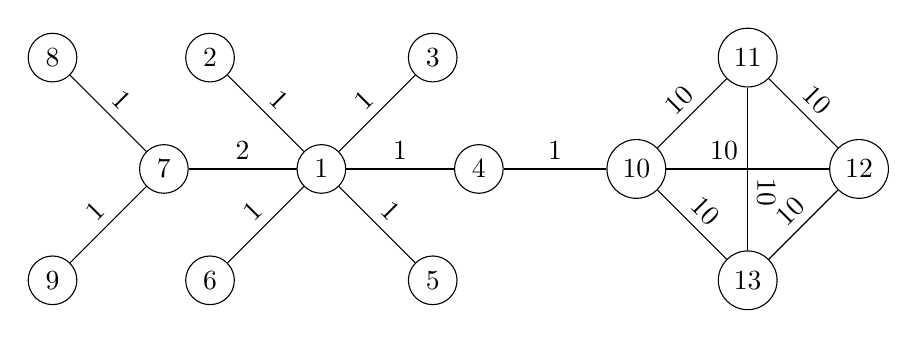
\begin{tikzpicture}[node distance=2cm]
        \node[circle, draw] (1) {1};
        \node[circle, draw] (2) [above left of=1] {2};
        \node[circle, draw] (3) [above right of=1] {3};
        \node[circle, draw] (4) [right of=1] {4};
        \node[circle, draw] (5) [below right of=1] {5};
        \node[circle, draw] (6) [below left of=1] {6};
        \node[circle, draw] (7) [left of=1] {7};
        
        \node[circle, draw] (8) [above left of=7] {8};
        \node[circle, draw] (9) [below left of=7] {9};

        \node[circle, draw] (10) [right of=4] {10};
        \node[circle, draw] (11) [above right of=10] {11};
        \node[circle, draw] (12) [below right of=11] {12};
        \node[circle, draw] (13) [below right of=10] {13};
        
        \draw (1) -- (2) node[midway, above, sloped] {1};
        \draw (1) -- (3) node[midway, above, sloped] {1};
        \draw (1) -- (4) node[midway, above, sloped] {1};
        \draw (1) -- (5) node[midway, above, sloped] {1};
        \draw (1) -- (6) node[midway, above, sloped] {1};
        \draw (1) -- (7) node[midway, above, sloped] {2};
        
        \draw (7) -- (8) node[midway, above, sloped] {1};
        \draw (7) -- (9) node[midway, above, sloped] {1};
        \draw (4) -- (10) node[midway, above, sloped] {1};

        \draw (10) -- (11) node[midway, above, sloped] {10};
        \draw (10) -- (12) node[midway, above left, sloped] {10};
        \draw (10) -- (13) node[midway, above, sloped] {10};
        \draw (11) -- (12) node[midway, above, sloped] {10};
        \draw (11) -- (13) node[midway, above right, sloped] {10};
        \draw (12) -- (13) node[midway, above, sloped] {10};
    \end{tikzpicture}
    \caption{Graph illustration for a case of local search algorithm bad instance}
    \label{fig:local-search-bad-instance-1}
\end{figure}

Here, the first vertex that will be taken to form the initial solution will be $1$ because 
$d(1) = 6$ is the maximum degree and the second vertex will be $7$ because it is the 
highest degree neighbor of $1$. This initial solution already forms a maximum clique of 
weight $2$. When we look at the neighbors of this solution by removing either $1$ or $2$, 
we will never obtain a better solution than the initial solution. However, we observe well 
on this example that the maximum clique is the clique formed by the vertices $\{10, 11, 12, 13\}$ 
of weight $60$, well higher than $2$. The best way to counter this kind of problem would be 
to use a \textbf{meta-heuristic algorithm} like grasp which will allow itself to take solutions 
of lesser quality to try to reach the best solution.
\bigskip

The second way in which the algorithm can make a bad choice at a given time is by incorrectly 
choosing which of the best neighbors of the current solution to keep. Let's take an example:

\begin{figure}[H]
    \centering
    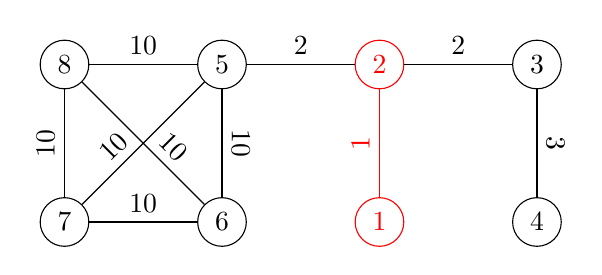
\begin{tikzpicture}[node distance=2cm]
        \node[circle, draw, red] (1) {1};
        \node[circle, draw, red] (2) [above of=1] {2};
        \node[circle, draw] (3) [right of=2] {3};
        \node[circle, draw] (4) [right of=1] {4};
        \node[circle, draw] (5) [left of=2] {5};
        \node[circle, draw] (6) [left of=1] {6};
        \node[circle, draw] (7) [left of=6] {7};
        \node[circle, draw] (8) [above of=7] {8};

        \draw[red] (1) -- (2) node[midway, above, sloped] {1};
        \draw (2) -- (3) node[midway, above, sloped] {2};
        \draw (2) -- (5) node[midway, above, sloped] {2};
        \draw (3) -- (4) node[midway, above, sloped] {3};
        \draw (5) -- (6) node[midway, above, sloped] {10};
        \draw (5) -- (7) node[midway, above left, sloped] {10};
        \draw (5) -- (8) node[midway, above, sloped] {10};
        \draw (6) -- (7) node[midway, above, sloped] {10};
        \draw (6) -- (8) node[midway, above right, sloped] {10};
        \draw (7) -- (8) node[midway, above, sloped] {10};
    \end{tikzpicture}
    \caption{Graph illustration for a second case of local search algorithm bad instance}
    \label{fig:local-search-bad-instance-2}
\end{figure}

Here, let us suppose that the current solution is $C = \{1, 2\}$. When the algorithm goes 
to look for a neighbor of this solution, it will have two possible choices, both offering 
the same quality of solution: $\{2, 3\}$ and $\{2, 5\}$. The problem arises if he chooses 
to go towards $\{2, 3\}$. In this case, the best solution that he can find will be $\{3, 4\}$ 
with a weight of $3$ whereas if he had gone towards $\{2, 5\}$, he would have obtained the 
maximum clique $\{5, 6, 7, 8\}$ with a weight $60$. Even if we say in the algorithm that he 
must go to the solution which has the vertices of higher degree, the problem remains the 
same if we add a vertex between the $2$ and the $5$.
\bigskip

But even if there are several possibilities for the algorithm not to act as we would like it 
to, as we said before the goal of a heuristic algorithm is not to find the best solution, but 
to find an approximate solution in a very short time compared to the exact algorithm.